%%%%%%%%%%%%%%%%%%%%%%%%%%%%%%%%%%%%%%%%%
% Lachaise Assignment
% LaTeX Template
% Version 1.0 (26/6/2018)
%
% This template originates from:
% http://www.LaTeXTemplates.com
%
% Authors:
% Marion Lachaise & François Févotte
% Vel (vel@LaTeXTemplates.com)
%
% License:
% CC BY-NC-SA 3.0 (http://creativecommons.org/licenses/by-nc-sa/3.0/)
% 
%%%%%%%%%%%%%%%%%%%%%%%%%%%%%%%%%%%%%%%%%

%----------------------------------------------------------------------------------------
%	PACKAGES AND OTHER DOCUMENT CONFIGURATIONS
%----------------------------------------------------------------------------------------

\documentclass{article}
\bibliographystyle{IEEEtran}
\usepackage[utf8]{inputenc}
\usepackage[english]{babel}
\usepackage{graphicx}
\usepackage[parfill]{parskip}
%%%%%%%%%%%%%%%%%%%%%%%%%%%%%%%%%%%%%%%%%
% Lachaise Assignment
% Structure Specification File
% Version 1.0 (26/6/2018)
%
% This template originates from:
% http://www.LaTeXTemplates.com
%
% Authors:
% Marion Lachaise & François Févotte
% Vel (vel@LaTeXTemplates.com)
%
% License:
% CC BY-NC-SA 3.0 (http://creativecommons.org/licenses/by-nc-sa/3.0/)
% 
%%%%%%%%%%%%%%%%%%%%%%%%%%%%%%%%%%%%%%%%%

%----------------------------------------------------------------------------------------
%	PACKAGES AND OTHER DOCUMENT CONFIGURATIONS
%----------------------------------------------------------------------------------------

\usepackage{amsmath,amsfonts,stmaryrd,amssymb} % Math packages

\usepackage{enumerate} % Custom item numbers for enumerations

\usepackage[ruled]{algorithm2e} % Algorithms

\usepackage[framemethod=tikz]{mdframed} % Allows defining custom boxed/framed environments

\usepackage{listings} % File listings, with syntax highlighting
\lstset{
	basicstyle=\ttfamily, % Typeset listings in monospace font
}

%----------------------------------------------------------------------------------------
%	DOCUMENT MARGINS
%----------------------------------------------------------------------------------------

\usepackage{geometry} % Required for adjusting page dimensions and margins

\geometry{
	paper=a4paper, % Paper size, change to letterpaper for US letter size
	top=2.5cm, % Top margin
	bottom=3cm, % Bottom margin
	left=2.5cm, % Left margin
	right=2.5cm, % Right margin
	headheight=14pt, % Header height
	footskip=1.5cm, % Space from the bottom margin to the baseline of the footer
	headsep=1.2cm, % Space from the top margin to the baseline of the header
	%showframe, % Uncomment to show how the type block is set on the page
}

%----------------------------------------------------------------------------------------
%	FONTS
%----------------------------------------------------------------------------------------

\usepackage[utf8]{inputenc} % Required for inputting international characters
\usepackage[T1]{fontenc} % Output font encoding for international characters

\usepackage{XCharter} % Use the XCharter fonts

%----------------------------------------------------------------------------------------
%	COMMAND LINE ENVIRONMENT
%----------------------------------------------------------------------------------------

% Usage:
% \begin{commandline}
%	\begin{verbatim}
%		$ ls
%		
%		Applications	Desktop	...
%	\end{verbatim}
% \end{commandline}

\mdfdefinestyle{commandline}{
	leftmargin=10pt,
	rightmargin=10pt,
	innerleftmargin=15pt,
	middlelinecolor=black!50!white,
	middlelinewidth=2pt,
	frametitlerule=false,
	backgroundcolor=black!5!white,
	frametitle={Command Line},
	frametitlefont={\normalfont\sffamily\color{white}\hspace{-1em}},
	frametitlebackgroundcolor=black!50!white,
	nobreak,
}

% Define a custom environment for command-line snapshots
\newenvironment{commandline}{
	\medskip
	\begin{mdframed}[style=commandline]
}{
	\end{mdframed}
	\medskip
}

%----------------------------------------------------------------------------------------
%	FILE CONTENTS ENVIRONMENT
%----------------------------------------------------------------------------------------

% Usage:
% \begin{file}[optional filename, defaults to "File"]
%	File contents, for example, with a listings environment
% \end{file}

\mdfdefinestyle{file}{
	innertopmargin=1.6\baselineskip,
	innerbottommargin=0.8\baselineskip,
	topline=false, bottomline=false,
	leftline=false, rightline=false,
	leftmargin=1cm,
	rightmargin=1cm,
	singleextra={%
		\draw[fill=black!10!white](P)++(0,-1.2em)rectangle(P-|O);
		\node[anchor=north west]
		at(P-|O){\ttfamily\mdfilename};
		%
		\def\l{3em}
		\draw(O-|P)++(-\l,0)--++(\l,\l)--(P)--(P-|O)--(O)--cycle;
		\draw(O-|P)++(-\l,0)--++(0,\l)--++(\l,0);
	},
	nobreak,
}

% Define a custom environment for file contents
\newenvironment{file}[1][File]{ % Set the default filename to "File"
	\medskip
	\newcommand{\mdfilename}{#1}
	\begin{mdframed}[style=file]
}{
	\end{mdframed}
	\medskip
}

%----------------------------------------------------------------------------------------
%	NUMBERED QUESTIONS ENVIRONMENT
%----------------------------------------------------------------------------------------

% Usage:
% \begin{question}[optional title]
%	Question contents
% \end{question}

\mdfdefinestyle{question}{
	innertopmargin=1.2\baselineskip,
	innerbottommargin=0.8\baselineskip,
	roundcorner=5pt,
	nobreak,
	singleextra={%
		\draw(P-|O)node[xshift=1em,anchor=west,fill=white,draw,rounded corners=5pt]{%
		Question \theQuestion\questionTitle};
	},
}

\newcounter{Question} % Stores the current question number that gets iterated with each new question

% Define a custom environment for numbered questions
\newenvironment{question}[1][\unskip]{
	\bigskip
	\stepcounter{Question}
	\newcommand{\questionTitle}{~#1}
	\begin{mdframed}[style=question]
}{
	\end{mdframed}
	\medskip
}

%----------------------------------------------------------------------------------------
%	WARNING TEXT ENVIRONMENT
%----------------------------------------------------------------------------------------

% Usage:
% \begin{warn}[optional title, defaults to "Warning:"]
%	Contents
% \end{warn}

\mdfdefinestyle{warning}{
	topline=false, bottomline=false,
	leftline=false, rightline=false,
	nobreak,
	singleextra={%
		\draw(P-|O)++(-0.5em,0)node(tmp1){};
		\draw(P-|O)++(0.5em,0)node(tmp2){};
		\fill[black,rotate around={45:(P-|O)}](tmp1)rectangle(tmp2);
		\node at(P-|O){\color{white}\scriptsize\bf !};
		\draw[very thick](P-|O)++(0,-1em)--(O);%--(O-|P);
	}
}

% Define a custom environment for warning text
\newenvironment{warn}[1][Warning:]{ % Set the default warning to "Warning:"
	\medskip
	\begin{mdframed}[style=warning]
		\noindent{\textbf{#1}}
}{
	\end{mdframed}
}

%----------------------------------------------------------------------------------------
%	INFORMATION ENVIRONMENT
%----------------------------------------------------------------------------------------

% Usage:
% \begin{info}[optional title, defaults to "Info:"]
% 	contents
% 	\end{info}

\mdfdefinestyle{info}{%
	topline=false, bottomline=false,
	leftline=false, rightline=false,
	nobreak,
	singleextra={%
		\fill[black](P-|O)circle[radius=0.4em];
		\node at(P-|O){\color{white}\scriptsize\bf i};
		\draw[very thick](P-|O)++(0,-0.8em)--(O);%--(O-|P);
	}
}

% Define a custom environment for information
\newenvironment{info}[1][Info:]{ % Set the default title to "Info:"
	\medskip
	\begin{mdframed}[style=info]
		\noindent{\textbf{#1}}
}{
	\end{mdframed}
}


%----------------------------------------------------------------------------------------
%	ASSIGNMENT INFORMATION
%----------------------------------------------------------------------------------------

\title{Cluster and Cloud Computing Assignment 2
		\\ City Analytic on the Cloud} % Title of the assignment

\author{ Zhaofeng Qiu \texttt{1101584}} % Author name and email address

\date{University of Melbourne --- \today} % University, school and/or department name(s) and a date

%----------------------------------------------------------------------------------------

\begin{document}

\maketitle % Print the title

%----------------------------------------------------------------------------------------
%	INTRODUCTION
%----------------------------------------------------------------------------------------

\section{System Design and Architecture}
The architecture of our system is well designed. It is aimed to provide both a beautiful front-end web application and a RESTFul API server with high availability, high scalability, and fault tolerance. The overall architecture is shown in Figure \ref{fig:systemArchitecturePsystemArchitecture}. 

\begin{figure}[htp]
\centering
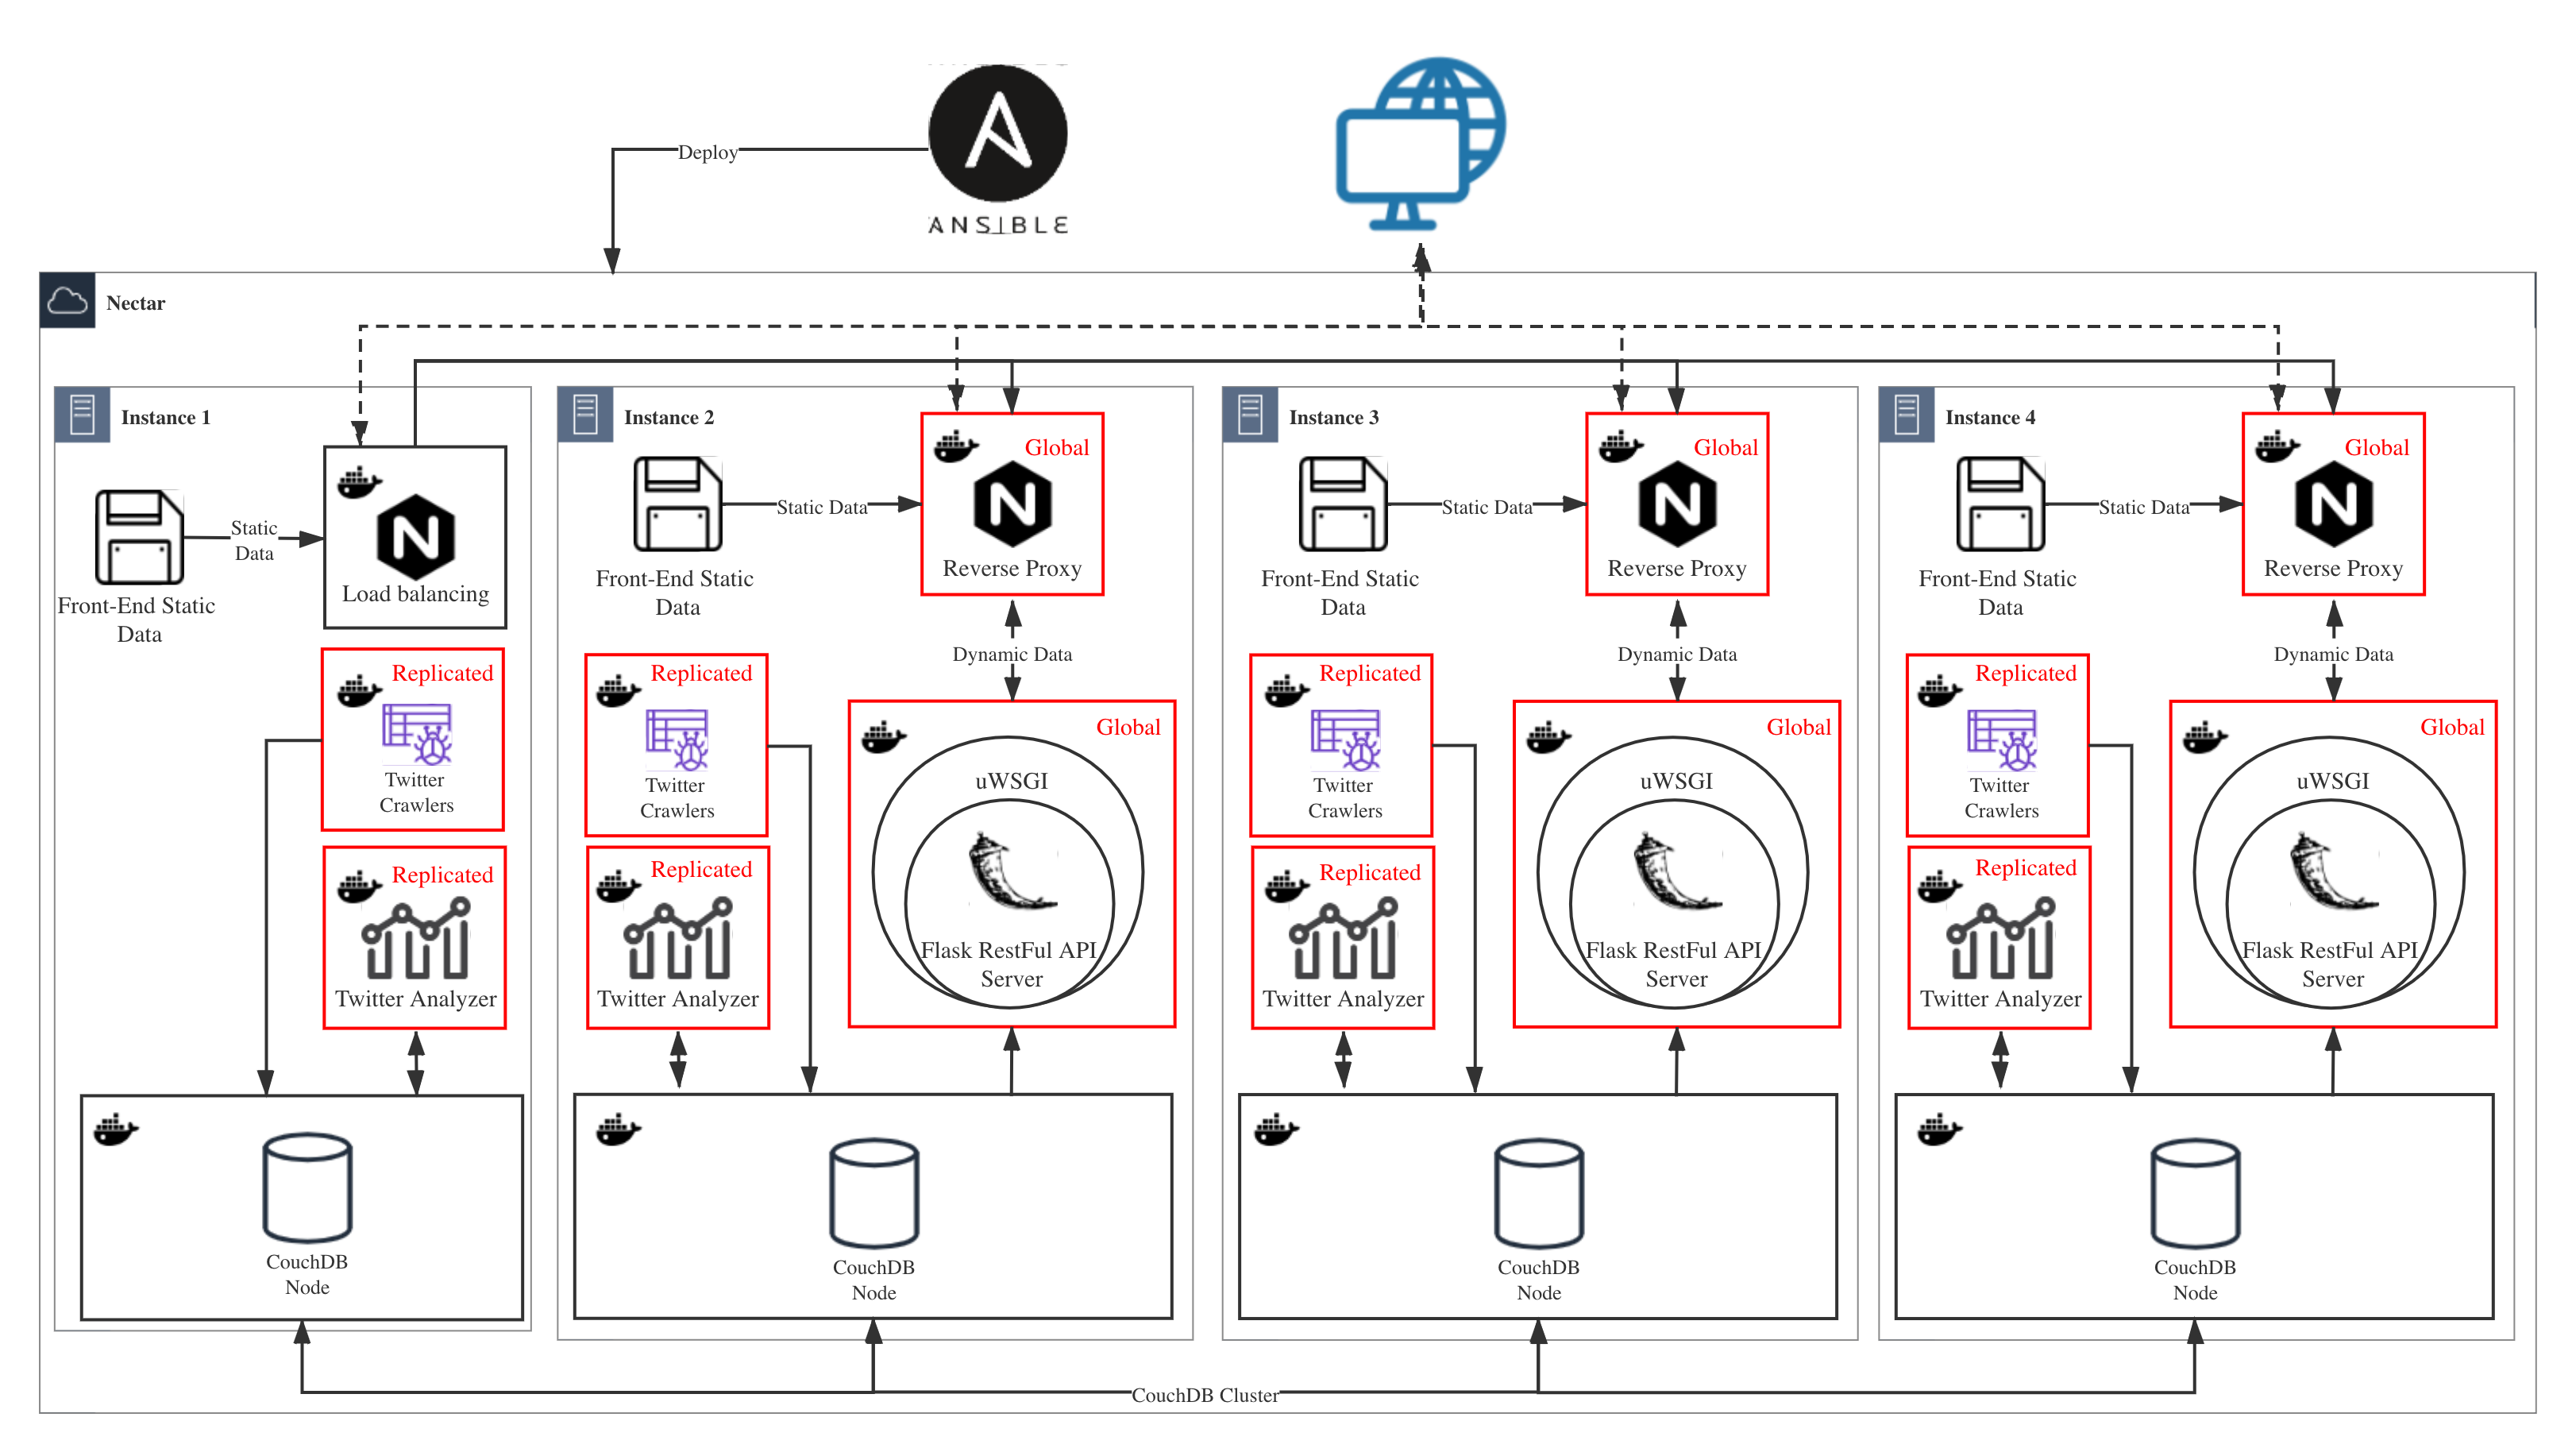
\includegraphics[width=\textwidth]{img/architecture.png}
\caption{Velocity Re-estimation}
\label{fig:systemArchitecturePsystemArchitecture}
\end{figure}

\subsection{Availability}
We continue to optimize our architecture through in-depth thinking and repeated practice to improve the availability of our system with limited resources.

Firstly, we run an \textit{Nginx} server in our first instance to provide Load balancing. For requests that need to access the dynamic data in our database, it would pass the request to the other three servers averagely. In this way, we can efficiently distribute the incoming network traffic to our backend servers in the cluster. When it comes to the situation where the first instance may crash, users can still access our application through the IPs of the other three nodes. However, this solution is not good enough and is contradict to high availability. We had tried to use two \textit{Nginx} server with a software called Keepalived to provide a more fault-tolerant system. However, we found out that we are not allowed to use floating IP in \textit{Nectar}. Since we cannot set a virtual IP for our \textit{Nginx} servers, the only way to handle this issue is to let the other three nodes to keep the full functionality of our application. Users can access our application through any IP of our instances, but only the IP of the first instance would provide load balancing control. 

Secondly, we use \textit{Docker Swarm} to manage part of our services. The containers which are in red boxes in Figure \ref{fig:systemArchitecturePsystemArchitecture} are managed by \textit{Docker Swarm}. The containers that with a "global" deploy mode setting would run in each of our machines except Instance 1. The containers with a "replicated" deploy mode setting would run in one of the four nodes. Actually, we have twelve \textit{Twitter} Crawlers in our cluster, each for different purposes. They would be distributed to different nodes in our cluster by \textit{Docker Swarm}. The \textit{Docker Swarm} does not manage the \textit{CouchDB} container and the Load Balancing \textit{Nginx} server. But they can restart themselves if they crush since we set the "restart" configuration in docker-compose to "always". We didn't include the \textit{CouchDB} into the \textit{Swarm} cluster because using \textit{Swarm} to manage the \textit{CouchDB} database could be counter-productive if the \textit{Swarm} manager deploys two \textit{CouchDB} together to the same node. The Load balancing \textit{Nginx} server is also not included because its port number is in conflict with the reverse proxy \textit{Nginx} server in the \textit{Docker Swarm} network. We set three \textit{Swarm} manager nodes in our cluster. Any instance with an ID bigger than three would be set to be a worker node. A single leader is elected from the three \textit{Swarm} manager nodes to conduct our orchestration tasks. Our manager would also run the services as worker nodes. According to \cite{pros-and-cons-of-running-all-docker-swarm-nodes-as-managers} and \textit{Swarm} Admin Guide\footnote{https://docs.docker.com/engine/swarm/admin\_guide/}, the number of our manager nodes is set based on the following facts:
\begin{itemize}
	\item More managers would result in a longer election for a new leader when one goes down. The \textit{Swarm} is in a read-only state which means that no new replica tasks can be launched and no service can be updates. No auto-recover can happen during the election.
	\item More managers would require tighter management of resources to prevent manager starvation.
	\item Fewer managers would increase the probability of all managers going down.
	\item To support manager node failures, the number of managers should be an odd number and should bigger than one. In our cluster, we can only provide four nodes. So, setting the number of managers to be three in our system is our best choice. In this way, our system can provide fault tolerance that one of our manager nodes can crash.
\end{itemize}

Hello everyone! Here I am going to introduce our Cluster and Cloud Computing gourp project.
 

Thirdly, we use a \textit{CouchDB} cluster with four nodes to improve our system's availability. We keep three replicas in our cluster, which means that any two nodes can be down in our system without crashing down our application. The Flask RESTFul API server, the \textit{Twitter} Crawler, and the \textit{Twitter} Analyzer of our system would only access the \textit{CouchDB} database in their localhost. In this way, errors on a single node will not affect other nodes. 

In conclusion, our system is a fault-tolerant system. Our application could run well even if two nodes in our cluster crashed. Except for the first node, any node in our system can provide all the services we need to run our front-end web application and RESTFul API server themselves. The system can be easily improved to a real high availability system by adding one more Load balancing \textit{Nginx} server and using Keepalived to manage the floating IP system.

\subsection{Dynamic and Static Separation}
We use \textit{Nginx} to separate static from dynamic traffic. For accessing the static data on our websites like HTML and image files, the \textit{Nginx} server would handle them itself. For accessing the dynamic data from the database, the reverse proxy \textit{Nginx} server passes the request to the uWSGI-Flask server through socket protocol. When using a socket, external browsers will not be able to directly access our uWSGI-Flask service, which can provide additional safety. It is faster to transfer through the socket. There are many advantages to separate static traffic. For one thing, it can help reduce the file I/O and storage consumption of our uWSGI-Flask server. \textit{Nginx} is good at handling static traffic, which can provide a quick response to our front-end application. Further more, we can reuse the RESTFul API in our front-end application to reduce workload.

\subsection{Scalability}
We use Ansible to deploy our system. To add more nodes into the cluster or change some settings of the instance, we can change a few variables in our Ansible playbook and deploy them by a few commands. Instead of running all the playbook, we can run some specific tasks to save the deployment time since we also set the tags of our tasks on the Ansible playbook properly. Docker Swarm is used to providing self-healing and Rolling updates. The core docker images of our system have been published to Docker Hub. We can update our system by asking the Docker Swarm to pull the new images and use a rolling update to deploy a new version system. The Ansible playbook is well designed, using many new features of Ansible. We use many variables in our Ansible playbook to provide a better scale-up experience instead of hard coding.



%%%%%%%%%%% May be useful in the future:%%%%%%%%%%%%%%%%%%

% \begin{file}[2nodes8cores.slurm]
% \begin{lstlisting}[]
% code
% \end{lstlisting}
% \end{file}


% \begin{file}[docker service ls (brief)]
% \begin{lstlisting}[]
% NAME                         MODE                REPLICAS      
% app_\textit{nginx}_app                global              3/3           
% app_rESTful_api_server       global              3/3             
% app_tweet_analyzer           replicated          1/1             
% app_tweet_hist               replicated ˜         1/1             
% app_tweet_hist_Adelaide      replicated          1/1             
% app_tweet_hist_Brisbane      replicated          1/1             
% app_tweet_hist_Melbourne     replicated          1/1             
% app_tweet_hist_Perth         replicated          1/1             
% app_tweet_hist_Sydney        replicated          1/1             
% app_tweet_stream             replicated          1/1             
% app_tweet_stream_Adelaide    replicated          1/1             
% app_tweet_stream_Brisbane    replicated          1/1             
% app_tweet_stream_Melbourne   replicated          1/1             
% app_tweet_stream_Perth       replicated          1/1             
% app_tweet_stream_Sydney      replicated          1/1 
% \end{lstlisting}
% \end{file}

\bibliography{lib}
\end{document}
